\label{par:contrib1:stab}
L'objectif est d'appréhender la viabilité des ImEx ARK sur l'équation de Nagumo. Dans ce but, leur stabilité est étudiée.
Dans un premier temps, une étude générale de la stabilité des ImEx ARK est menée.
Puis, l'étude de stabilité se centre sur l'application à l'équation de Nagumo. L'ensemble des codes utilisés pour évaluer numériquement et afficher les domaines de stabilités
sont disponibles à l'adresse: \href{https://github.com/Ocelot-Pale/ImEx_stability_Nagumo}{https://github.com/Ocelot-Pale/ImEx\_stability\_Nagumo}.



\subsubsection{Étude de stabilité générale des RK-ImEx}
    Avec une méthode ImEx, les deux opérateurs de l'EDP sont découplés, c'est là l'intérêt.
    Cependant cela complexifie l'analyse usuelle de stabilité. 
    En effet la fonction de stabilité attend alors deux variables, 
    le coefficient spectral $Z_E$ associé à l'opérateur traité explicitement et
    le coefficient spectral $Z_I$ associé à l'opérateur traité implicitement.
    Ainsi, pour chaque couple $(Z_E,Z_I)$ d'indices spectraux, la fonction de stabilité prend une valeur différente, et comme les coefficients spectraux sont des nombres complexes, 
    on ne peut plus visualiser d'un simple coup d'oeil le domaine de stabilité, puisque celui-ci se trouve dans un espace de dimension quatre $\mathbb{C}^2$.
    % \footnote{En effet la fonction de stabilité $R \mathbb C \times \mathbb C \rightarrow \mathbb R$ et $\dim  \mathbb C \times \mathbb C=4$.}.
    \paragraph{Calcul des fonctions d'amplification }
    Afin d'étudier la stabilité linéaire des méthodes, les fonctions d'amplifications ont été évaluées numériquement.
    L'algorithme est le suivante:
    \begin{enumerate}
        \item Entrer les valeurs de $(Z_E,Z_I)$ pour lesquelles la fonction de stabilité doit être évaluée
        \item Simuler un pas du schéma en partant de $u_0 = 1$ appliqué à une équation du type Dahlquist :\\$\dt{u} = \lambda_E u + \lambda_I u$
        \begin{enumerate}
            \item Construire toutes les approximations intermédiaires avec les valeurs 
            \item Construire l'approximation finale $u_1$
        \end{enumerate}
        \item Évaluer la norme de $u_1$
    \end{enumerate}
    Cette l'étude générale, c'est à dire pour tout $(Z_E,Z_I) \in \mathbb{C}^2$ n'est pas détaillée ici, toutefois
    le lecteur intéressé pourra trouver les graphiques représentants les domaines de stabilité sur le \href{https://github.com/Ocelot-Pale/ImEx_stability_Nagumo}{Notebook en ligne}.


\subsubsection{Étude de stabilité linéaire appliquée à l'équation de Nagumo}
    La démarche précédente est particularisée en se centrant sur l'équation de Nagumo ; 
    permettant d'étudier la stabilité des méthodes ImEx sur ce problème particulier.
    \paragraph{Valeurs propres mises en jeu}
        Comme expliqué en \ref{par:analyser_operateurs_nagumo} l'équation présente deux opérateurs : 
        \begin{itemize}
            \item[$\diamond$] La diffusion dont le spectre s'étend de $\frac{-1}{L^2}$ à $\frac{-1}{\Delta x^2}$ (où $L$ est la taille du domaine discrétisé).
            \item[$\diamond$] La réaction dont le spectre balaie continûment $-k$ jusqu'à $2k$
        \end{itemize}
        Pour particulariser l'analyse de stabilité il faut donc tracer le diagramme de stabilité des méthodes étudiées en prenant $Z_I \in \mathbb{R}^-$ 
        et $Z_E \in [-k;2k] \subset \mathbb{R}$ ce qui donne un espace à deux dimensions. Il est ensuite pertinent placer des couples $(Z_E,Z_I)$ correspondant.
        Cela donne les diagrammes en fig. \ref{fig:stabilite_nagumo}
    \paragraph{Résultats}
    \begin{figure}[htbp]
        \centering
        
        \begin{subfigure}{\textwidth}
            \centering
            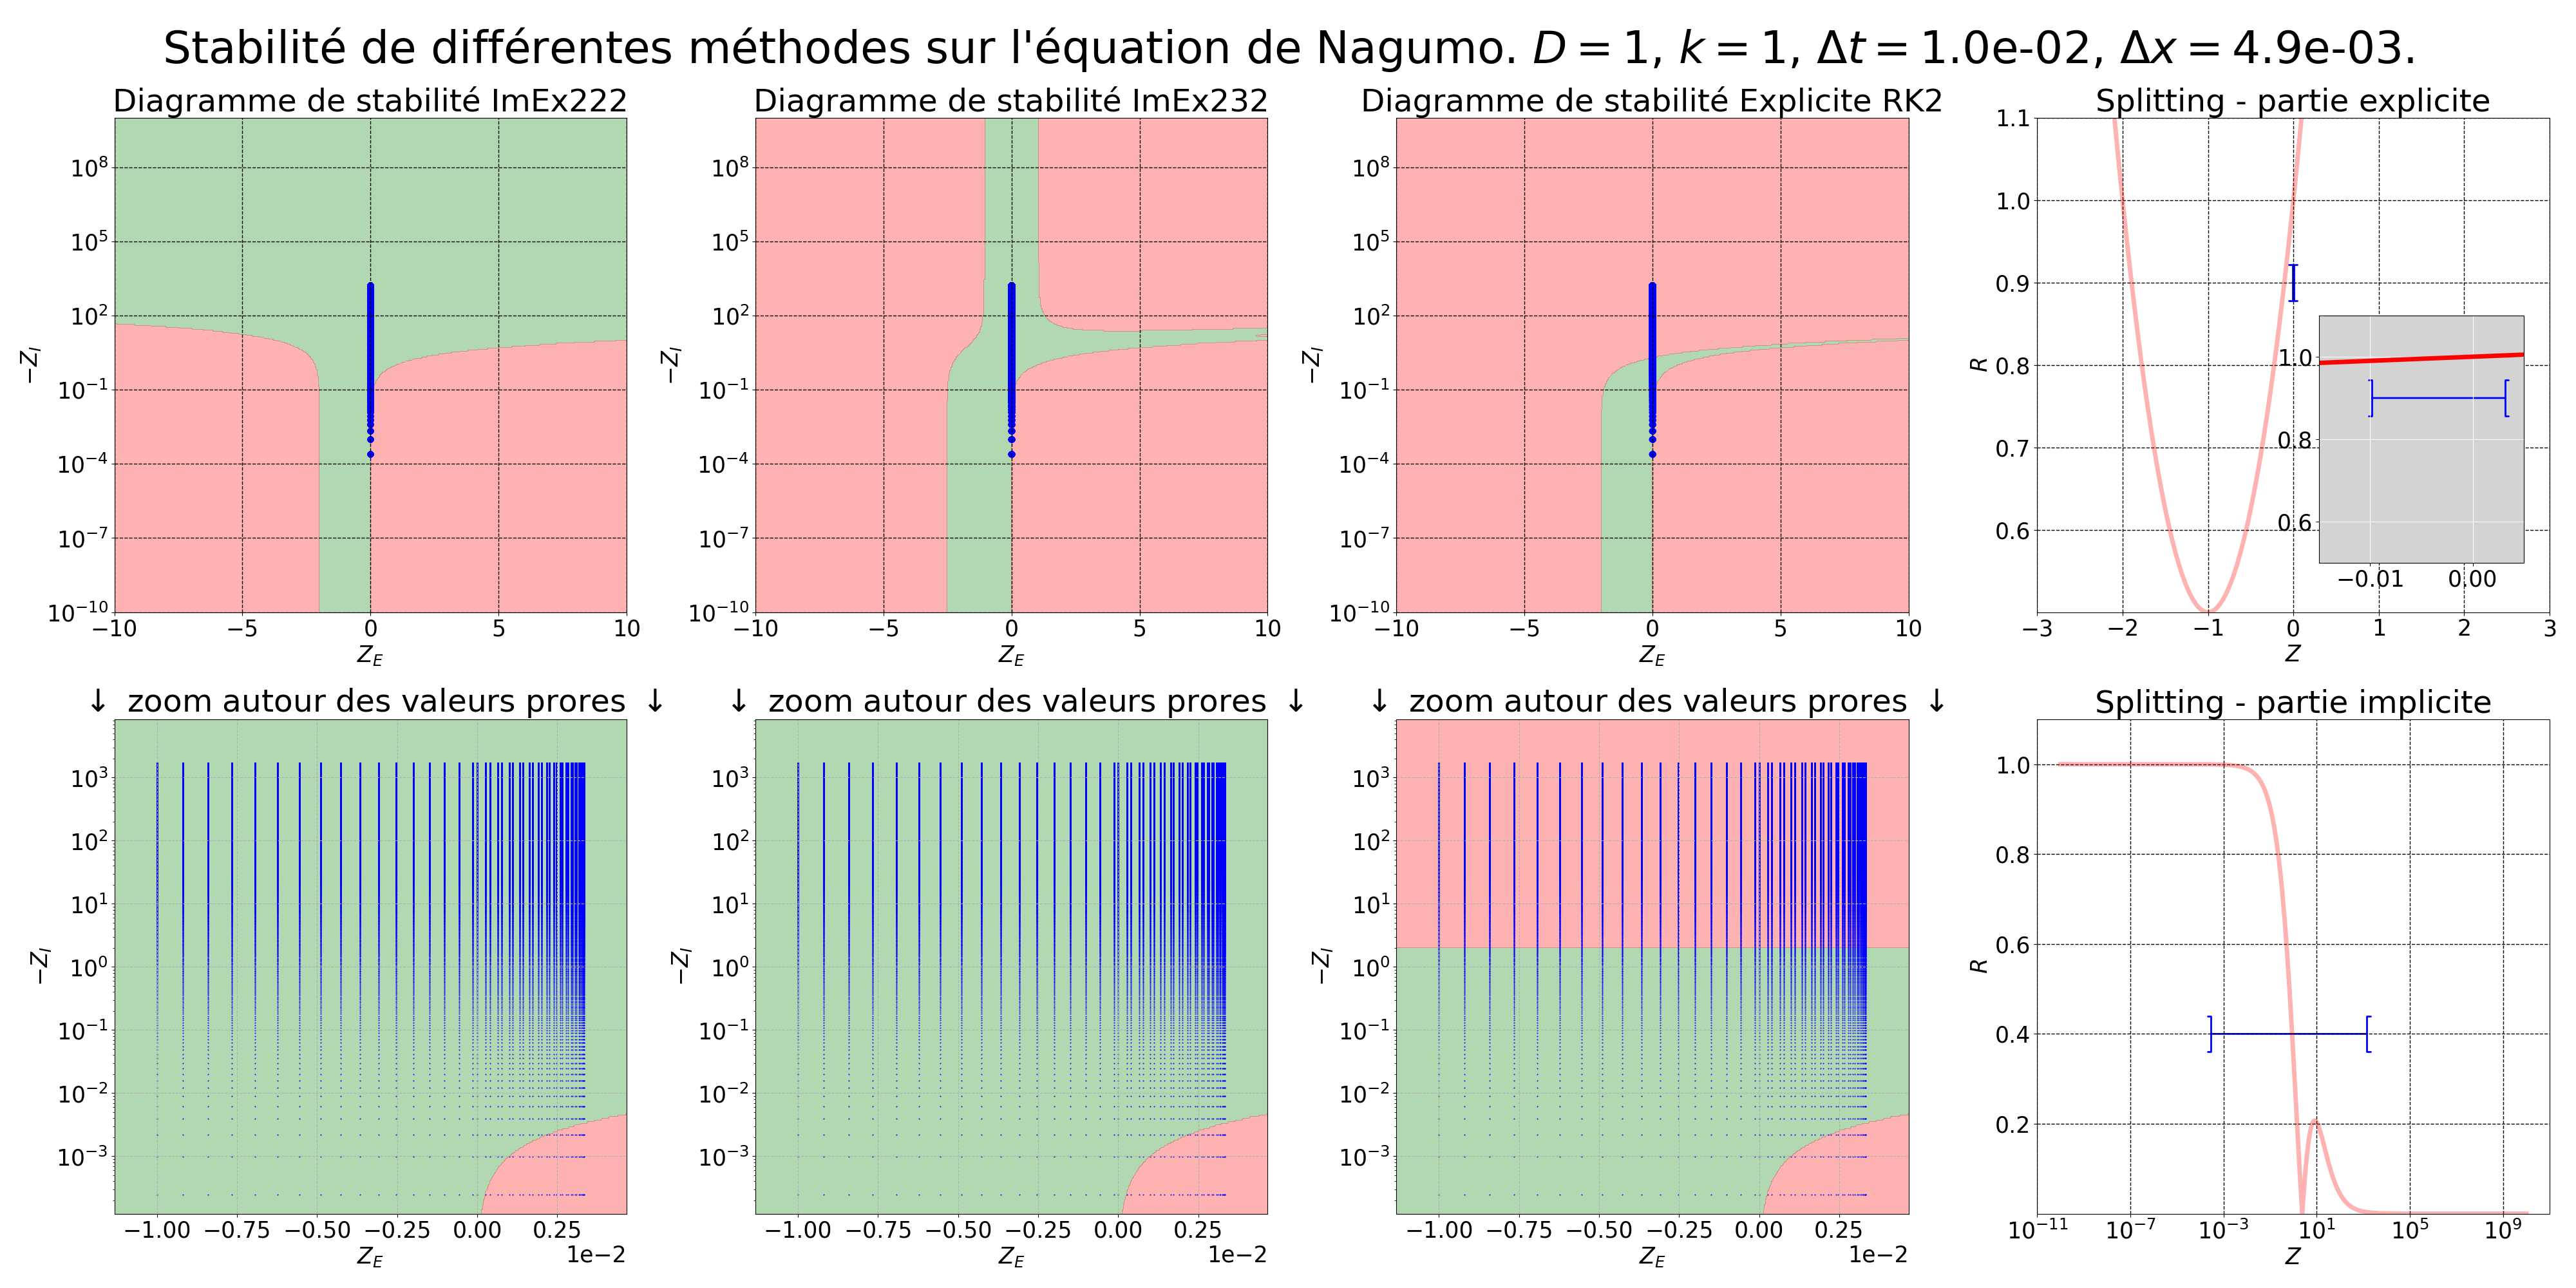
\includegraphics[width=0.8\textwidth]{media/4_travail/2_nagumo/stabilite/STABILITE_D1_k1_dt1.0e-02_dx4.9e-03.png}
            \caption{Cas standard\\D=1, k=1, dt=1.0e-03, dx=2.4e-03}
            \label{fig:stabilite_nagumo_a}
        \end{subfigure}
        
        \vspace{0.5cm} % Espacement entre les sous-figures
        
        \begin{subfigure}{\textwidth}
            \centering
            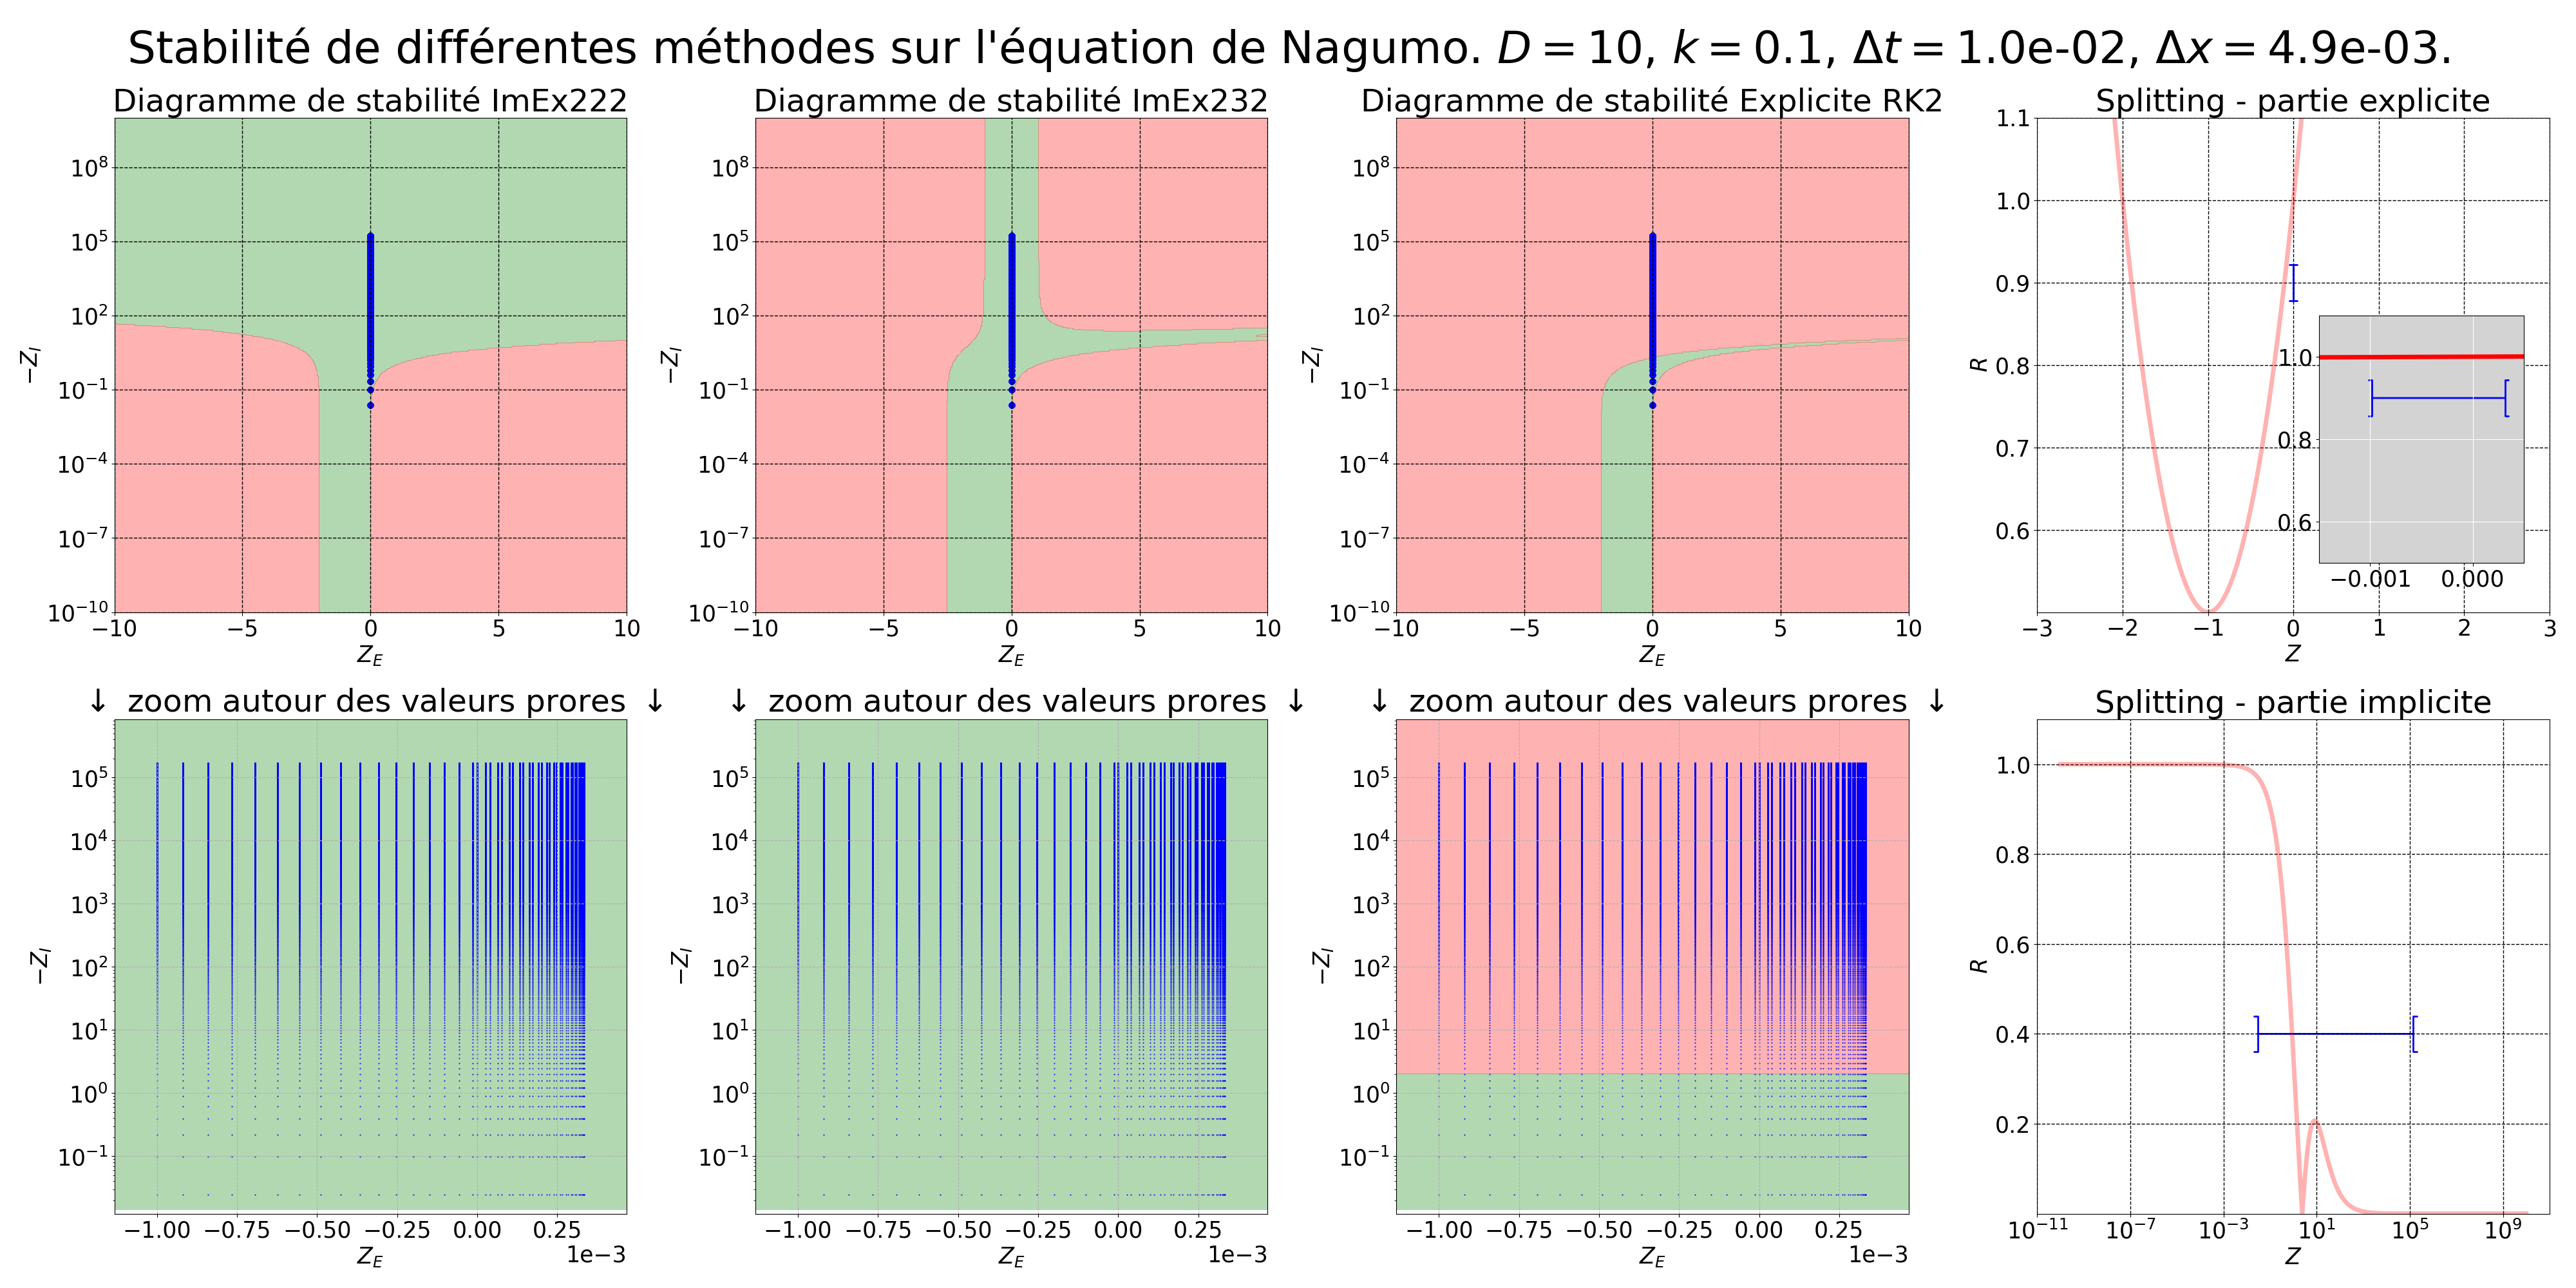
\includegraphics[width=0.8\textwidth]{media/4_travail/2_nagumo/stabilite/STABILITE_D10_k0.1_dt1.0e-02_dx4.9e-03.png}
            \caption{Cas diffusion plus raide, réaction moins raide\\D=10, k=0.1, dt=1.0e-02, dx=4.9e-03}
            \label{fig:stabilite_nagumo_b}
        \end{subfigure}

        \begin{subfigure}{\textwidth}
            \centering
            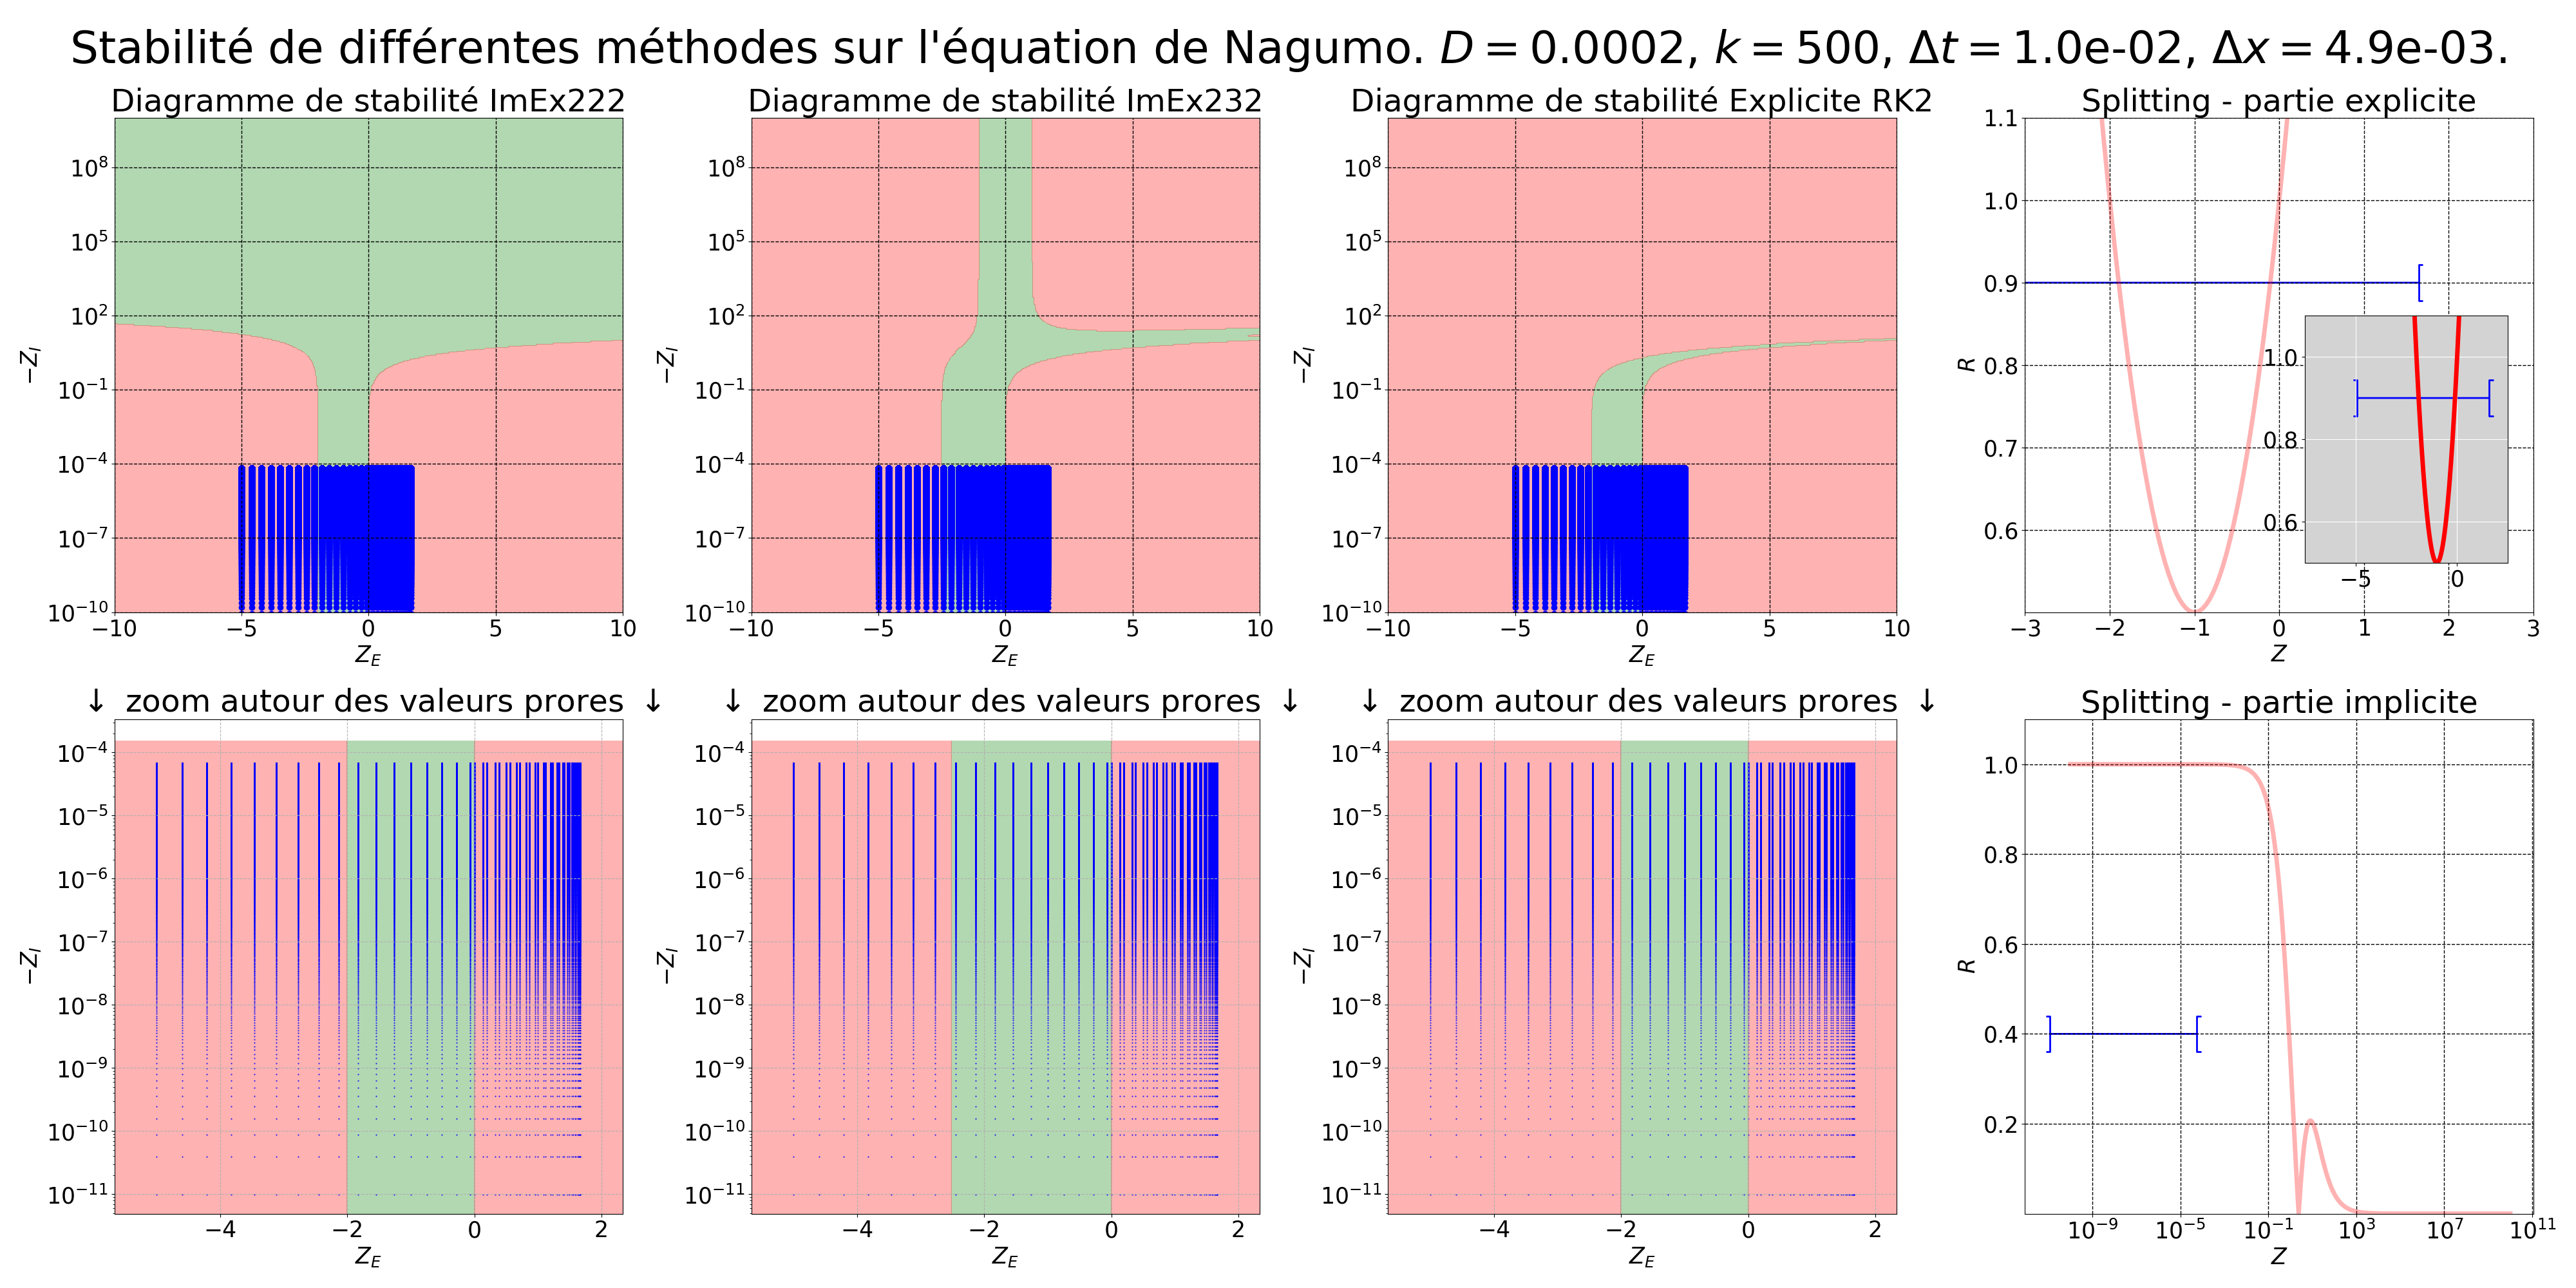
\includegraphics[width=0.8\textwidth]{media/4_travail/2_nagumo/stabilite/STABILITE_D0.0002_k500_dt1.0e-02_dx4.9e-03.png}
            \caption{Cas diffusion moins raide, réaction plus raide\\D=2e-4, k=500, dt=1.0e-02, dx=4.9e-03}
            \label{fig:stabilite_nagumo_c}
        \end{subfigure}
        
        \caption{Diagrammes de stabilité des méthodes ImEx comparés à ceux d'une méthode explicite à un schéma de splitting sur l'équation de Nagumo, pour différents couples $D$ et $k$.}
        \label{fig:stabilite_nagumo}
    \end{figure}
        Ces diagrammes permettent d'analyser respectivement la stabilité de la méthode \emph{ImEx222}, de la méthode \emph{ImEx232},
        et, à titre de comparaison, la stabilité d'une méthode \emph{Runge et Kutta explicite} d'ordre 2\footnote{Celle apparaissant dans ImEx222.} 
        et d'un \emph{schéma de splitting de Strang} utilisant une RK explicite pour la réaction et une RK implicite pour la diffusion.
        Chaque colonne représente l'analyse d'une méthode différente.
        \begin{itemize}
        \item[$\diamond$] La première ligne présente le domaine de stabilité en fonction des indices spectraux $Z_E \in \mathbb{R}$ et $Z_I \in \mathbb{R}^-$.
        \item[$\diamond$] La seconde ligne est un zoom  autour de ces indices spectraux.
        \item[$\diamond$] Les points bleus représentent les couples d'indices spectraux intervenant dans la résolution de l'équation de Nagumo
        pour les paramètres d'équation choisis ($D$ et $k$) et les paramètres de discrétisation retenus ($\Delta t$ et $\Delta x$).
        
        \item[$\diamond$] La dernière colonne (splitting) présente une disposition différente, puisque les opérateurs sont totalement découplés.
            \begin{itemize}
                \item[$\diamond$] La première ligne correspond alors à la fonction de stabilité de la méthode explicite (avec un zoom autour des indices spectraux de la réaction) et
                \item[$\diamond$] la seconde ligne représente la fonction de stabilité de la méthode implicite. 
                \item[$\diamond$] Dans les deux cas, l'intervalle tracé en bleu représente la plage de valeurs d'indices spectraux balayés par chaque opérateur.
            \end{itemize}
        \end{itemize}
        \paragraph{Analyse}
            \subparagraph{Analyse générale}\label{par:analyse_generale_stab_nagumo}
                Analyse des domaines de stabilité (fig.\figref{fig:stabilite_nagumo}) :
                \begin{itemize}
                    \item[$\diamond$]\textbf{Méthode explicite:} En troisième colonne, le diagramme de stabilité d'une méthode explicite RK explicite d'ordre deux, sert de référence. 
                        Le domaine de stabilité s'étend pour des indices spectraux négatifs jusqu'à $-2$ (résultat classique des méthodes EKR2).
                        Le schéma traitant conjointement les deux opérateurs, l'indice spectral résultant est $Z=Z_E+Z_I$. 
                        De fait domaine de stabilité s'étend jusqu'à $-2$ selon l'axe $Z_E$ tant que $Z_I$ est négligeable et de même,
                        le domaine de stabilité s'étend jusqu'à $-2$ selon $Z_I$ tant que $Z_E$ est négligeable. 
                        Enfin il y a une zone intermédiaire où $Z_E$ et $Z_I$ sont tous les deux de l'ordre de l'unité\footnote{Attention à l'échelle logarithmique.}.

                    \item[$\diamond$]\textbf{Méthode ImEx232:} La seconde colonne montre que la méthode ImEx232 maintient un domaine de stabilité restreint (jusqu'à $-2$) selon l'axe $Z_E$,
                        mais présente un domaine de stabilité bien plus étendu selon l'axe $Z_I$.
                        C'est logique puisque la valeurs propre $Z_E$ est explicitée,
                        sont domaine pris seul n'a évolué, et la valeur propre $Z_I$ peut être très raide (très négative) puisque la méthode traite explicitement l'opérateur lié à $Z_I$.
                        % Voir que le domaine de stabilité est légèrement décalé vers la droite quand $Z_I$ est grand

                    \item[$\diamond$]\textbf{Méthode ImEx222:} Passant à la première colonne, le domaine de stabilité ImEx222 resemble beaucoup à celui de l'ImEx232.
                        Néanmoins, le domaine de stabilité de l’épateur explicité est considérablement élargit 
                        là où $Z_I$ est assez grand. Cette propriété est remarquable : cela signifie que la stabilité de méthode ImEx résulte d'un couplage des raideurs ;
                        contrairement au splitting qui, par nature, découple totalement les problématiques stabilités.
                        Plus précisément, plus l'opérateur implicité est raide, plus l'opérateur explicité peut être raide.
                        % AFAIRE :
                        % Pourquoi ? Qu'est ce qui change fondamentalement ? 
                        % ---> certaines VP positives ont une fonction d'amplification négatives pour la réaction, ca pourrait poser problème (perte d'ordre ?)
                        % justement pour le splitting c'est pas le cas, et lui il ne perd pas l'ordre ??? ... 
                \end{itemize}
            \subparagraph{Dépendance de la stabilité aux paramètres de l'équation $k$ et $D$}
                Grace au graphiques en \figref{fig:stabilite_nagumo} la disposition couples de valeurs 
                propres mis en jeu par l'équation de Nagumo peut être analysées selon les paramètre $k$ et $D$.\\
                \textbf{Contexte : }
                Les paramètres de simulation: $\Delta t$ et $\Delta x$ sont fixés.
                Les couples de paramètres choisis sont : $(k,D)=(1,1)$, $(k,D)=(0.1,10)$, $(k,D)=(500,2\, 10^{-4})$. 
                Le produit $kD$ est maintenu égal à un, ainsi la vitesse de propagation est toujours la même (\emph{cf.} \ref{par:analyser_operateurs_nagumo}).
                Ces couples de valeurs propres $Z_E,Z_I$ sont en effet tracés en bleus sur le graphique
                \footnote{Pour $Z_E$, le spectre est continu, il a donc fallut échantillonnés le long de l'axe $Z_E$}.\\
                \textbf{Analyse : }
                \begin{itemize}
                    \item[$\diamond$]\textbf{Cas standard, $(k,D)=(1,1)$} - \figref{fig:stabilite_nagumo_a}:\\
                        Dans ce cas, la raideur de la diffusion déstabilise la méthode RKE2 (de nombreux indices spectraux tombent dans le zones rouges à cause des grandes valeurs de $Z_I$).
                        Pour ces valeurs de $(\Delta x, \Delta t)$ cette méthode n'est donc pas stable.
                        C'est ce qui est attendu, les méthodes explicite imposent des pas de temps très restrictifs sur les problèmes de diffusion.

                        En revanche, les méthodes ImEx sont stables puisque le domaine de stabilité est infini vers $Z_I \rightarrow -\infty$.
                        Certains couples de valeurs propres tombent malgré tout dans une zone instable (en bas à gauche). En réalité ce n'est pas un problème car il s'agit 
                        de couples où l'indice spectral $Z_E$ associé à l'opérateur de réaction est positif. Donc ce n'est est pas vraiment une instabilité, la méthode elle reflète simplement
                        la dynamique explosive de la réaction. D'ailleurs le graphique de la méthode explicite du splitting, il y a une zone 
                        où la fonction d'amplification est d'amplitude supérieure à un, le splitting reproduit donc fidèlement la dynamique de la réaction.
                        En revanche,
                        pour les méthodes ImEx, il existe des couples de d'indice spectraux propres où $Z_E$ est positif alors que la fonction d'amplification est d'amplitude inférieure à un. 
                        Cela pourrait être un frein pour reproduire fidèlement la dynamique explosive de la réaction dans les zones concernées
                        \footnote{Il n'est pas évident d'avoir \textit{a priori} la bonne intuition car peut être que la diffusion calme en quelque sorte 
                        le caractère explosif de la réaction et qu'alors une fonction d'amplification d'amplitude $< 1$ est normal...}.
                    \item[$\diamond$]\textbf{Cas diffusion raide, réaction peu raide, $(k,D)=(0.1,10)$}  - \figref{fig:stabilite_nagumo_b}:\\
                        Ici, $D=10$ donc toutes les valeurs propres liées à la diffusion sont multipliées par 10 par rapport au cas précédent. 
                        De fait la méthode RK2E de référence présente des instabilités pour encore plus de couples de valeurs propres est n'est pas pas viable.
                        Concernant les méthodes ImEx222 et ImEx232 elles restent stables, et cette fois-ci tous les couples d'indices spectraux liés à la 
                        dynamique explosive de la réaction sont amortie ce qui n'est pas forcément incohérent puisque la diffusion domine.
                        % ---> AFAIRE voir expérimentalement ce que ça donne... 
                    \item[$\diamond$]\textbf{Cas diffusion peu raide, réaction très raide$(k,D)=(500,2\, 10^{-4})$} - \figref{fig:stabilite_nagumo_c}\\
                        Dans ce cas de figure, $k=500$. La grande valeur du coefficient de réaction rend cette dernière très raide. 
                        Cela a pour effet de dilater les couples d'indices spectraux selon l'axe des abscisse puisque $Z_E \in [- 500 \Delta t, + 1000 \Delta t]$
                        alors que pour $k=1$: $Z_E \in [- \Delta t , 2\Delta t]$.
                        Ici la méthode explicite au sein des ImEx n'est plus stable pour la réaction, ainsi toutes les méthodes deviennent instables. 
                        Le splitting également devient instable car il utilise aussi la méthode RK2E pour la réaction. 
                        Le fait que la méthode explicite de l'ImEx soit instable pour l'opérateur explicité peu sembler un obstacle infranchissable,
                        cependant ce n'est pas si simple.
                        Pour illustrer ce point, étendons l'analyse avec le cas spécial en \figref{fig:stabilite_nagumo_cas_special}, dans ce cas la réaction est toujours raide $k=500$ mais la diffusion est également très raide car $D=500$
                        \footnote{Jusqu'ici, la vitesse de propagation était la même dans tous les scénarios puisque $kD$ était maintenu constant. Dans le scénario présenté ici, ce n'est plus le cas}
                        Alors la méthode ImEx222 devient stable, comme vu en \ref{par:analyse_generale_stab_nagumo}, plus l'opérateur traité implicitement est raide, 
                        plus la méthode permet à l'opérateur traité explicitement d'être raide. C'est un cas remarquable ou le couplage intervenant au sein de la méthode ImEx
                        la rend plus stable que le splitting !
                \end{itemize}
                \begin{figure}[htbp]
                    \centering
                    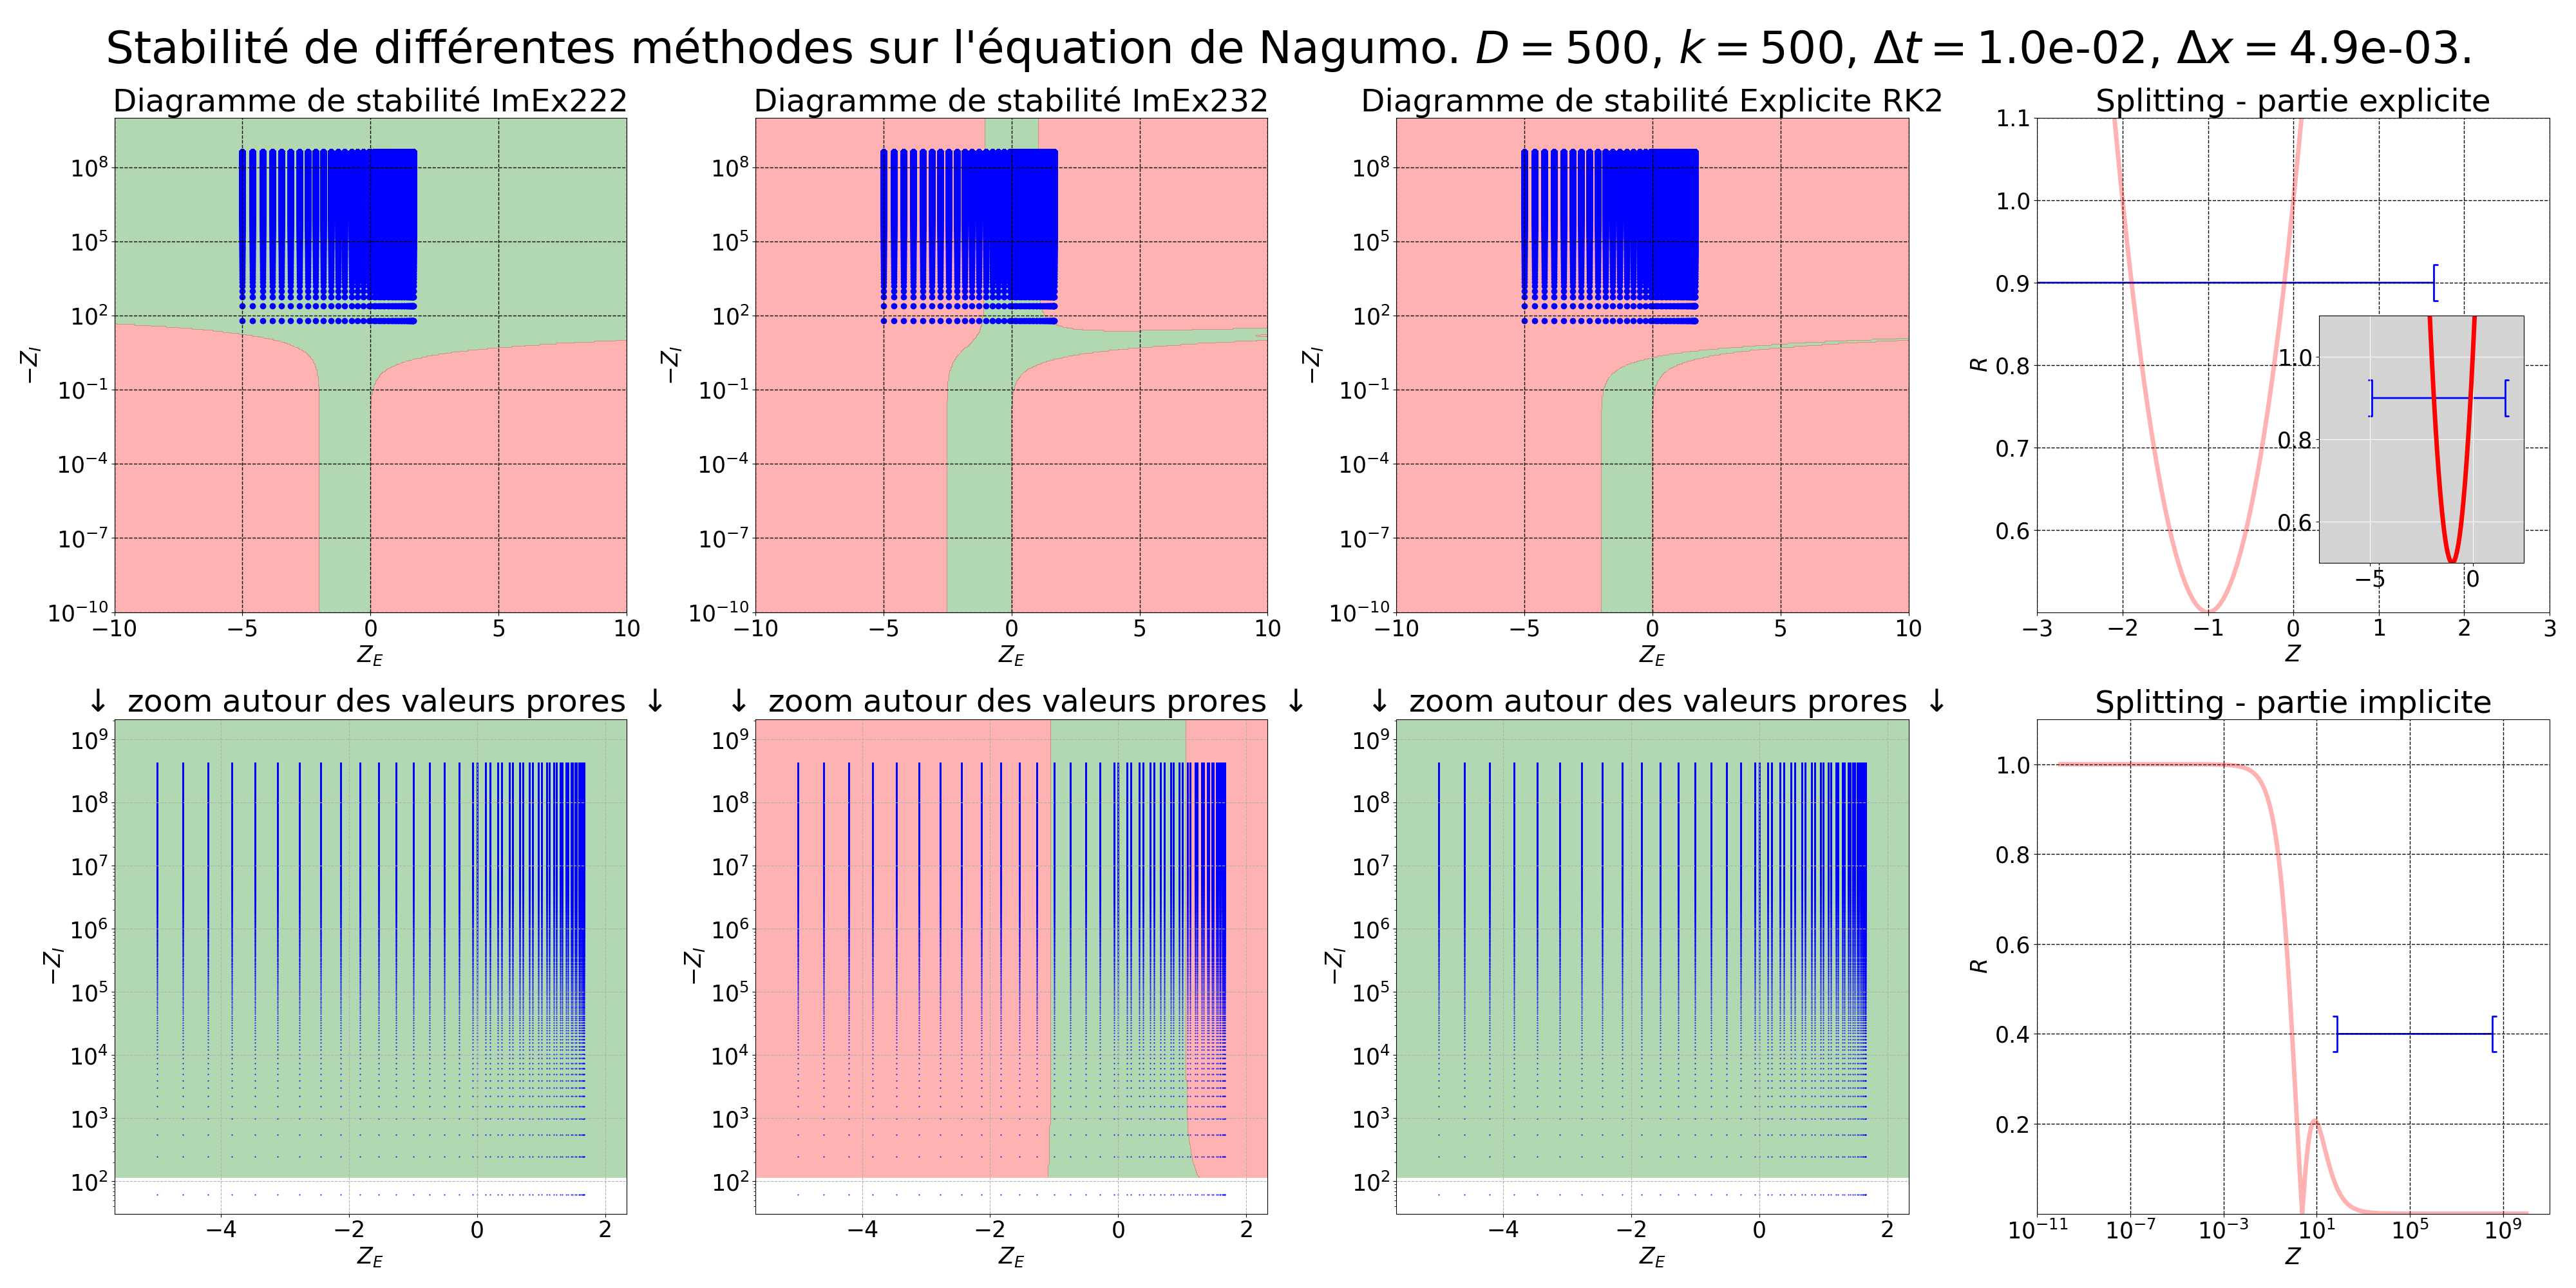
\includegraphics[width=0.8\textwidth]{media/4_travail/2_nagumo/stabilite/STABILITE_D500_k500_dt1.0e-02_dx4.9e-03.png}
                    \caption{Pour $k=500$ et $D=500$: diagrammes de stabilité des méthodes ImEx et de référence sur l'équation de Nagumo.}
                    \label{fig:stabilite_nagumo_cas_special}
                \end{figure}
            % \subparagraph{Analyse selon les paramètres de simulation $\Delta t$ et $\Delta x$}
                